\cleardoublepage
\chapter{HASIL SURVEI LAPANGAN DAN WAWANCARA}

\section{Transkrip dan Catatan Wawancara Operasional Bus Listrik TransJogja}

Wawancara dilakukan dengan pihak operator TransJogja (PT AMI) untuk memahami kondisi operasional riil (\textit{as-is}) armada bus listrik. Berikut adalah rangkuman hasil wawancara berdasarkan catatan dan rekaman lapangan:

\subsection*{Latar Belakang dan Infrastruktur}
\begin{itemize}
    \item Dinas Perhubungan (Dishub) DIY menggunakan Dana Keistimewaan untuk membeli 2 unit bus listrik pada tahun 2024. Setelah proses kalibrasi rute, bus tersebut ditugaskan kepada operator PT AMI pada 17 Januari 2025.
    \item Pemilihan lokasi SPKLU pertama di Terminal Adisucipto didasarkan pada kepemilikan lahan (tanah milik Dishub DIY). Rencana pembangunan SPKLU di masa depan juga diprioritaskan pada aset lahan milik Dishub DIY.
\end{itemize}

\subsection*{Peta Jalan (\textit{Roadmap}) Elektrifikasi}
\begin{itemize}
    \item \textbf{Tahun 2025}: Uji coba koridor bertahap (3 bulan pertama Rute 1, 3 bulan kedua Rute 2, 3 bulan ketiga Rute 3, dan 3 bulan keempat Rute 4).
    \item \textbf{Tahun 2026}: Operasional resmi diluncurkan pada Rute L-1 (Terminal Jombor -- Malioboro -- Terminal Jombor).
    \item \textbf{Tahun 2027}: Direncanakan penambahan infrastruktur SPKLU di Terminal Jombor. Pihak operator juga telah mengajukan penambahan armada sebanyak 4 unit bus listrik kepada Dishub, meskipun realisasinya belum dipastikan. Penggunaan armada tambahan ini (apakah untuk memperkuat Rute L-1 atau membuka rute baru) akan bergantung pada hasil evaluasi ke depan.
\end{itemize}

\subsection*{Spesifikasi Kendaraan}
\begin{itemize}
    \item \textbf{Pabrikan/Karoseri}: PT MAB (Mobil Anak Bangsa), dengan karoseri New Armada.
    \item \textbf{Tipe}: Bus ukuran sedang (\textit{medium bus}).
    \item \textbf{Kapasitas Penumpang}: 28 orang (18 kursi duduk dan 10 ruang berdiri).
    \item \textbf{Kapasitas Baterai}: 127,74 -- 150 kWh.
    \item \textbf{Daya Jelajah}: Mampu menempuh jarak operasional hingga 150 km dalam sekali pengisian penuh.
    \item \textbf{Pengisian Daya}: Mendukung \textit{fast charging}. Kualitas baterai dijamin hingga 4.000 siklus pengisian (pengisian dari tingkat SoC mana pun ke 100\% dihitung sebagai 1 siklus). Arahan standar operasional adalah selalu mengisi daya hingga 100\% pada setiap sesi.
\end{itemize}

\subsection*{Kondisi Operasional Saat Ini (\textit{As-Is})}
\begin{itemize}
    \item Saat ini, 2 unit bus listrik beroperasi melayani Rute L-1 (Terminal Jombor -- Malioboro -- Terminal Jombor) dengan jam operasional pukul 05.30 hingga 20.30 WIB.
    \item Armada listrik ini berbasis di \textit{Pool} TransJogja Gamping.
    \item \textbf{Kinerja Pelayanan}: Bus melayani rata-rata 400 hingga 500 penumpang per hari. Waktu sibuk (\textit{peak hours}) terjadi pada pagi hari (sekitar pukul 09.00) dan sore hari (jam pulang kantor). Penumpang dapat memantau pergerakan bus secara \textit{real-time} melalui Aplikasi TransJogja.
    \item \textbf{Skema Bisnis}: Pembiayaan operasional bus listrik menggunakan sistem purnabayar (\textit{reimburse}) ke Dishub DIY.
    \item \textbf{Tanggapan Pengemudi}: Pengemudi melaporkan pengalaman berkendara yang lebih baik dan nyaman dibandingkan dengan bus diesel konvensional. Dari sisi mekanis, bus listrik juga membutuhkan perawatan yang jauh lebih sederhana.
\end{itemize}

\subsection*{Mekanisme Pengisian Daya dan Kendala Operasional}
\begin{itemize}
    \item Pengisian daya operasional dilakukan terpusat di SPKLU Adisucipto.
    \item Batas kritis kapasitas baterai (\textit{State of Charge} / SoC) ditetapkan pada 30\%. Di bawah 20\%, sistem kelistrikan sekunder (termasuk pendingin udara / AC) otomatis dimatikan oleh sistem.
    \item Jika bus mencapai batas minimum 30\% di tengah operasional, pengemudi diwajibkan menurunkan penumpang di halte terdekat (dalam cakupan Rute L-1), lalu menempuh perjalanan \textit{deadhead} (sekitar 30 menit) ke SPKLU Adisucipto. Waktu pengisian daya memakan waktu sekitar 1 jam, sehingga total waktu non-operasional mencapai 2 jam.
    \item Karena fleksibilitas ini, jadwal pengisian daya sangat bergantung pada penilaian pengemudi (\textit{driver behavior}).
    \item \textbf{Kendala Utama}: Kemacetan lalu lintas merupakan risiko tertinggi. Terdapat kekhawatiran bus mogok di tengah jalan karena tidak berhasil mencapai SPKLU sebelum kapasitas baterai terkuras habis (terkunci / sistem \textit{lock}).
\end{itemize}

\newpage
\section{Dokumentasi Survei Lapangan}

Berikut adalah beberapa foto dokumentasi yang diambil selama survei lapangan dan wawancara dengan pihak PT AMI (TransJogja):

\begin{figure}[h]
    \centering
    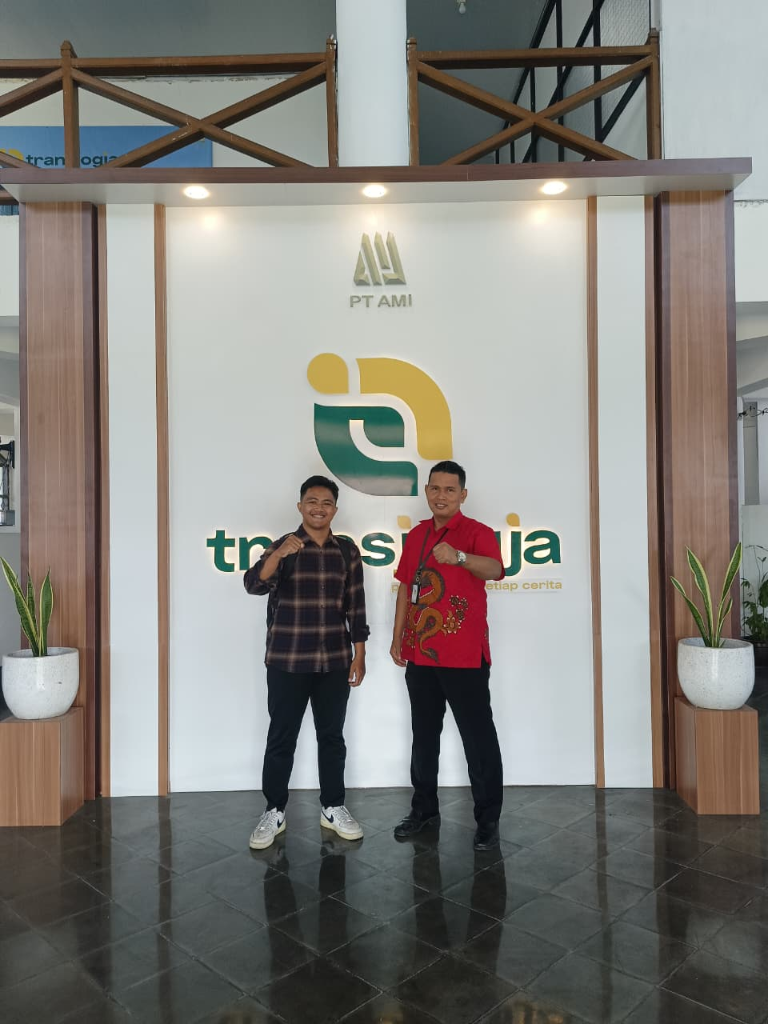
\includegraphics[width=0.6\linewidth]{images/wawancara-pt-ami.png}
    \caption{Wawancara di kantor operator PT AMI}
    \label{fig:survei-wawancara}
\end{figure}

\begin{figure}[h]
    \centering
    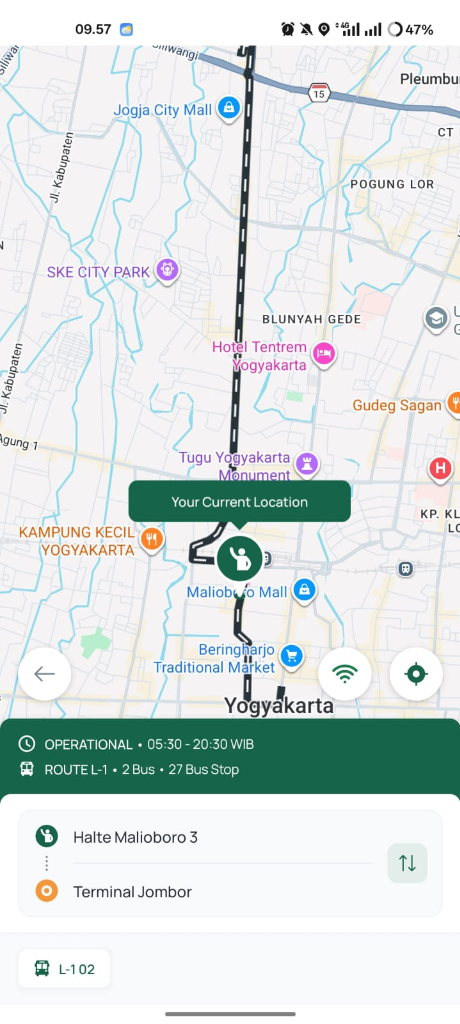
\includegraphics[width=0.5\linewidth]{images/aplikasi-transjogja.png}
    \caption{Pemantauan armada \textit{real-time} Rute L-1 pada aplikasi TransJogja}
    \label{fig:survei-app}
\end{figure}

\begin{figure}[h]
    \centering
    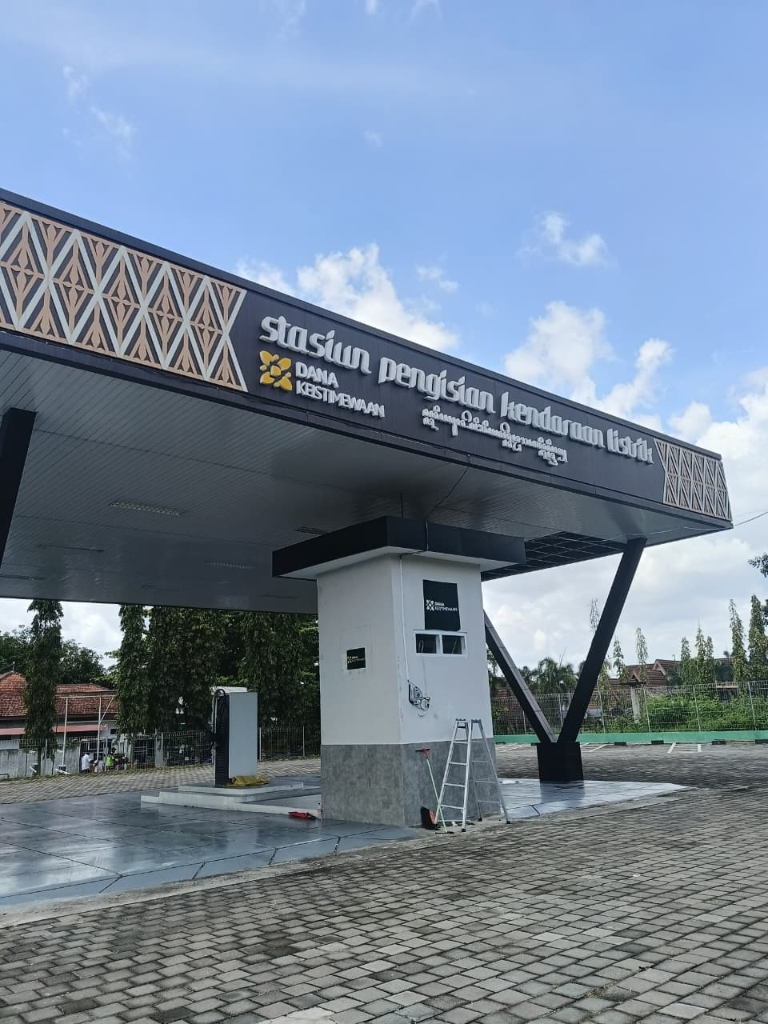
\includegraphics[width=0.6\linewidth]{images/spklu-adisucipto.jpg}
    \caption{Infrastruktur pengisian daya SPKLU di Terminal Adisucipto}
    \label{fig:survei-spklu}
\end{figure}

\begin{figure}[h]
    \centering
    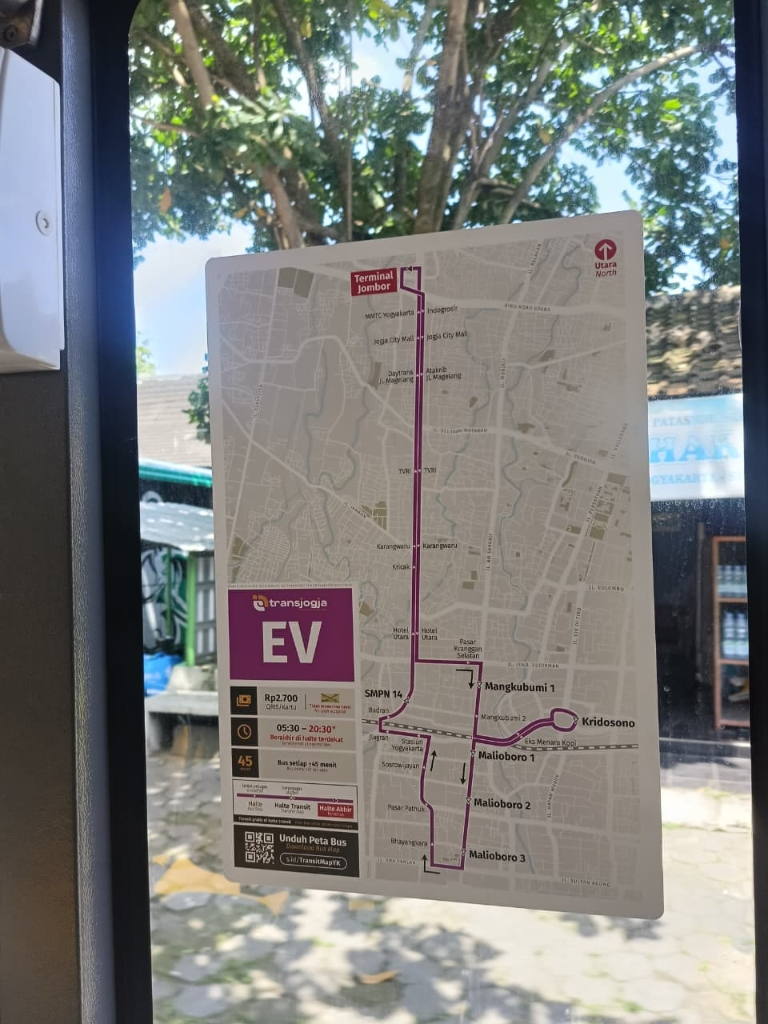
\includegraphics[width=0.5\linewidth]{images/peta-rute-bus.jpg}
    \caption{Peta informasi Rute L-1 (EV) di dalam armada bus listrik}
    \label{fig:survei-peta-rute}
\end{figure}

\begin{figure}[h]
    \centering
    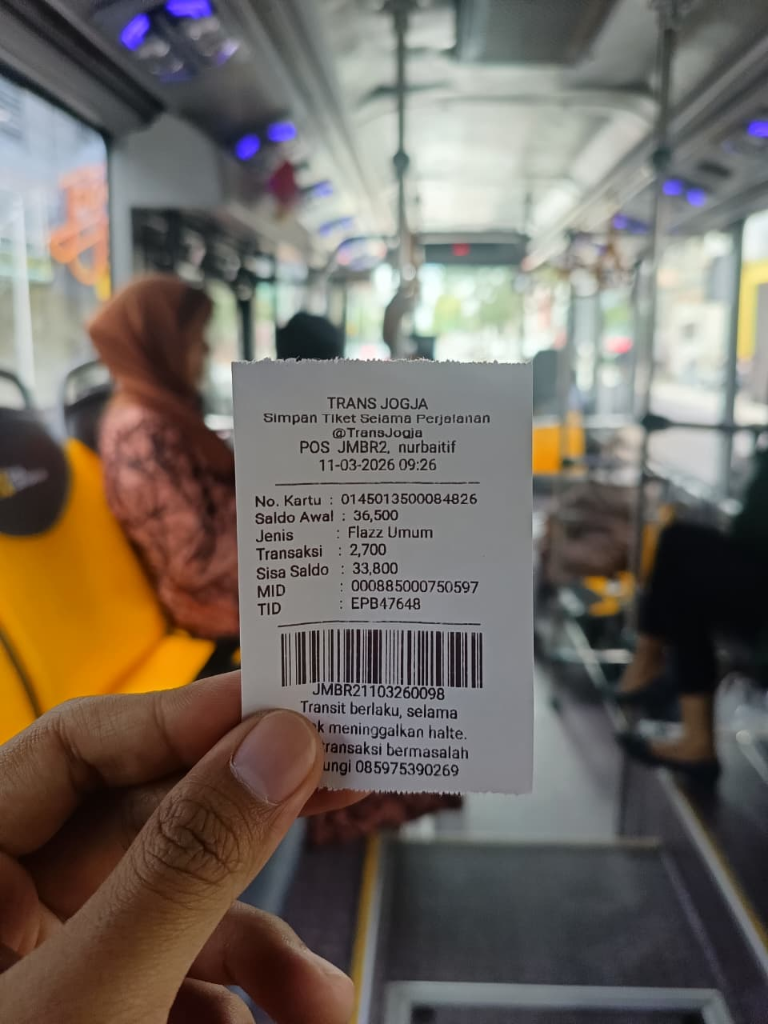
\includegraphics[width=0.5\linewidth]{images/tiket-transjogja.png}
    \caption{Tiket operasional TransJogja}
    \label{fig:survei-tiket}
\end{figure}
